Lorsque deux joueurs jouent à un jeu comme celui des amazones ou même des echecs,
les joueurs ont un but distinct. Imaginons une fonction $f(p, j)$ qui donne le score
d'un plateau $p$ pour le joueur $j$. Le joueur rouge tente de maximiser
$f(p, rouge)$ tandis que le joueur bleu tente de minimiser $f(p, rouge)$ et vice-versa.

C'est à partir de cette observation que l'algorithme minmax est conçu.

\subsubsection{L'algorithme minmax}
On peut représenter toutes les parties possibles comme un arbre de jeu.
\begin{figure}[H]
	\centering
	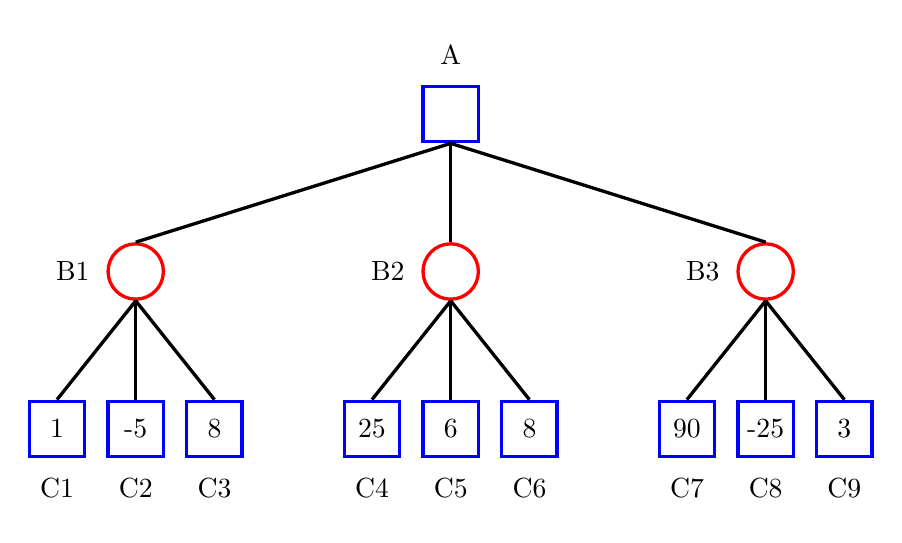
\begin{tikzpicture}
		\begin{scope}[every node/.style={draw=blue, minimum size=2em, very thick}]
			\node (A)[label=above:A] at (0,0) {};
			\node (C1)[label=below:C1] at (-5,-4) {1};
			\node (C2)[label=below:C2] at (-4,-4) {-5};
			\node (C3)[label=below:C3] at (-3,-4) {8};
			\node (C4)[label=below:C4] at (-1,-4) {25};
			\node (C5)[label=below:C5] at (0,-4) {6};
			\node (C6)[label=below:C6] at (1,-4) {8};
			\node (C7)[label=below:C7] at (3,-4) {90};
			\node (C8)[label=below:C8] at (4,-4) {-25};
			\node (C9)[label=below:C9] at (5,-4) {3};

		\end{scope}
		\begin{scope}[every node/.style={draw=red, circle, minimum size=2em, very thick}]
			\node (B1)[label=left:B1] at (-4,-2) {};
			\node (B2)[label=left:B2] at (0,-2) {};
			\node (B3)[label=left:B3] at (4,-2) {};
		\end{scope}
		\begin{scope}[every edge/.style={draw, very thick}]
			\path [-] (A.south) edge node {} (B1.north);
			\path [-] (A.south) edge node {} (B2.north);
			\path [-] (A.south) edge node {} (B3.north);
			\path [-] (B1.south) edge node {} (C1.north);
			\path [-] (B1.south) edge node {} (C2.north);
			\path [-] (B1.south) edge node {} (C3.north);
			\path [-] (B2.south) edge node {} (C4.north);
			\path [-] (B2.south) edge node {} (C5.north);
			\path [-] (B2.south) edge node {} (C6.north);
			\path [-] (B3.south) edge node {} (C7.north);
			\path [-] (B3.south) edge node {} (C8.north);
			\path [-] (B3.south) edge node {} (C9.north);
		\end{scope}
	\end{tikzpicture}
	\caption{Exemple d'arbre minmax pour un jeu quelconque}
	\label{fig:ex-minmax-debut}
\end{figure}

La figure~\ref{fig:ex-minmax-debut} montre un exemple de minmax à profondeur 3 sur un jeu où on peut jouer 3 coups différents sur un seul état.
Les carrés bleus représentent le joueur bleu, tandis que les cercles rouges représentent le joueur rouge.
Les feuilles seront toujours les seuls états évalués. Si on déroule l'algorithme, on obtient la figure~\ref{fig:ex-minmax-fin}.

\begin{figure}[H]
	\centering
	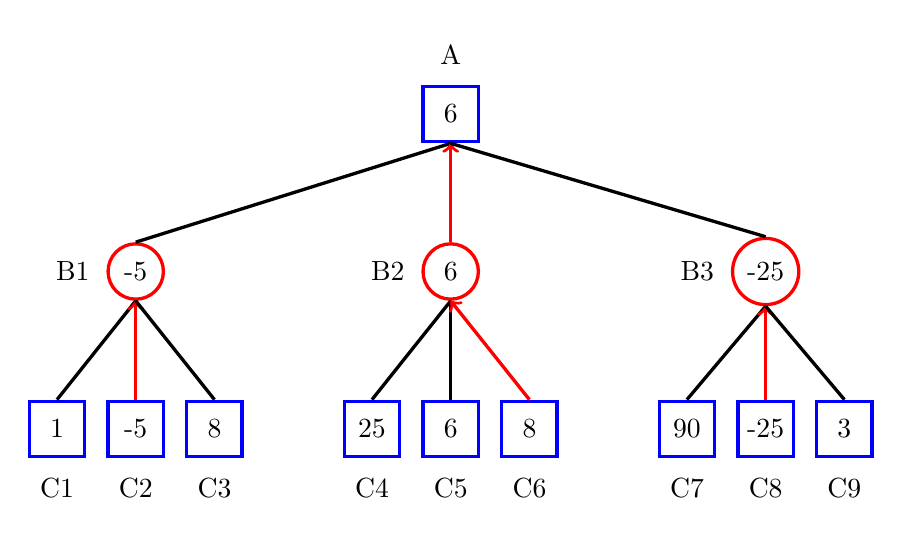
\begin{tikzpicture}
		\begin{scope}[every node/.style={draw=blue, minimum size=2em, very thick}]
			\node (A)[label=above:A] at (0,0) {6};
			\node (C1)[label=below:C1] at (-5,-4) {1};
			\node (C2)[label=below:C2] at (-4,-4) {-5};
			\node (C3)[label=below:C3] at (-3,-4) {8};
			\node (C4)[label=below:C4] at (-1,-4) {25};
			\node (C5)[label=below:C5] at (0,-4) {6};
			\node (C6)[label=below:C6] at (1,-4) {8};
			\node (C7)[label=below:C7] at (3,-4) {90};
			\node (C8)[label=below:C8] at (4,-4) {-25};
			\node (C9)[label=below:C9] at (5,-4) {3};

		\end{scope}
		\begin{scope}[every node/.style={draw=red, circle, minimum size=2em, very thick}]
			\node (B1)[label=left:B1] at (-4,-2) {-5};
			\node (B2)[label=left:B2] at (0,-2) {6};
			\node (B3)[label=left:B3] at (4,-2) {-25};
		\end{scope}
		\begin{scope}[every edge/.style={draw, very thick}]
			\path [-] (A.south) edge node {} (B1.north);
			\path [<-] (A.south) edge[draw=red] node {} (B2.north);
			\path [-] (A.south) edge node {} (B3.north);
			\path [-] (B1.south) edge node {} (C1.north);
			\path [<-] (B1.south) edge[draw=red] node {} (C2.north);
			\path [-] (B1.south) edge node {} (C3.north);
			\path [-] (B2.south) edge node {} (C4.north);
			\path [-] (B2.south) edge node {} (C5.north);
			\path [<-] (B2.south) edge[draw=red] node {} (C6.north);
			\path [-] (B3.south) edge node {} (C7.north);
			\path [<-] (B3.south) edge[draw=red] node {} (C8.north);
			\path [-] (B3.south) edge node {} (C9.north);
		\end{scope}
	\end{tikzpicture}
	\caption{Arbre minmax final après exécution de l'algorithme sur un jeu quelconque}
	\label{fig:ex-minmax-fin}
\end{figure}
Les noeuds rouges prennent la valeur minimale, tandis que le noeud bleu prend la valeur maximale.
D'après minmax, on devrait donc jouer le coup qui donne l'état B2. Cet algorithme
est exact. Cela veut dire que si on peut dérouler l'arbre complet des parties, on gagnera à coup sûr\footnote{Sauf si c'est un jeu non déterministe bien entendu}.
Mais, il est très improbable qu'on arrive à dérouler l'arbre des parties. En effet, pour un simple jeu où l'on ne
peut jouer que 3 coups par partie, à profondeur 3 l'algorithme évalue 9 noeuds. Pour un jeu où il y a $n$ coups possibles
par état, à une profondeur $d$, l'algorithme minmax calcule $n^{d-1}$ valeurs. Cela peut très vite exploser,
surtout quand le jeu en question est le jeu des amazones avec une cinquantaine de coups possibles selon le plateau.

Cependant, il existe une amélioration de minmax qui évite d'explorer des noeuds inutiles, l'élagage alpha-bêta.


\subsubsection{Amélioration de minmax: élagage alpha-beta}
L'élagage alpha-beta consiste à ne pas visiter de noeuds inutile. En effet, cet algorithme
profite du fait que le joueur rouge cherche à maximiser tandis que le joueur bleu cherche à minimiser.
Reprenons l'exemple en Figure~\ref{fig:ex-minmax-fin}.
Lorsque l'algorithme évalue B3, on cherche à maximiser, et le maximum courant est égal à 6.
Lorsqu'on évalue B3, on évalue d'abord C7 ce qui donne le score de 90, jusque là alphabeta ne fait rien.
Or, lorsqu'on évalue C8, la valeur est égale à -25. Cela veut-dire que la valeur de B3 est au moins
inférieure ou égale à -25. Or, le joueur bleu cherche à maximiser et possède un maximum courant égal à 6.
On sait donc que la valeur de A est au moins supérieure ou égale à 6. On peut en conclure que le noeud B3 sera de toute façon
moins bon que le noeud B2. On peut donc arrêter de l'explorer. Cet algorithme permet d'éviter d'explorer tous les noeuds. Malheureusement, la complexité
reste toujours exponentielle, mais elle reste meilleure que celle de minmax.

Théoriquement la complexité ne causerait pas de problèmes si nous avions
des ressources illimitées et du temps illimité. Or, nous n'avons pas ce luxe.
Sur le ladder\footnote{La plateforme où les différents clients des différentes équipes s'affrontent},
chaque joueur doit jouer tous ses coups en moins de 10s. Si on voulait passer largement
en dessous, il faudrait utiliser l'algorithme à profondeur 1. Or, cela n'est pas intéressant.
On peut tout de même prendre avantage du fait que l'arbre réduit massivement en taille plus la partie avance.
En effet, à chaque tour, une case en plus devient inaccessible. C'est pour cela
qu'on peut tout simplement choisir d'aller de plus en plus loin dans l'arbre des possibilités plus on
est loin dans la partie.

\subsubsection{Profondeur dynamique}
Comme énoncé précédemment, on prend avantage du fait que le jeu
se "simplifie" au cours du temps. On peut même en déduire que la partie
devient exponentiellement plus simple. Suite à beaucoup d'expérimentation,
nous avons déduit 2 méthodes principales pour déterminer la profondeur à jouer.
Une basée sur le temps passé à calculer un arbre alphabeta, et une basée
sur le nombre de tours.

\paragraph{Fonction de profondeur}
Comme fonction, nous avons décidé d'utiliser la fonction décrite dans l'équation~\ref{eq:deepening-function} où la fonction
$depth(t)$ retourne la profondeur voulue en fonction du nombre de tours écoulés $t$ et de la largeur du plateau $m$.
\begin{equation}
	depth(t) = \lfloor\exp\left(\frac{1.15*t}{\exp(0.05*m)*\sqrt{m}*m}\right)\rfloor
	\label{eq:deepening-function}
\end{equation}
Les paramètres ont été choisi relativement arbitrairement, mais nous avons tout de même
utilisé l'application Desmos\footnote{Une calculatrice graphique} qui nous a permis de mesurer
l'évolution de notre profondeur en fonction du nombre de tours. De plus, nous avons implémenté
le système de timeout sur notre serveur pour être sûr que notre algorithme ne prenait pas trop de temps.

\paragraph{Mesure du temps}
Ensuite, pour la deuxième façon d'augmenter la profondeur, le programme calcule
le temps maximal pour 1 tour ($\frac{timeout}{nombre\_cases}$),
mesure le temps pris pour une exécution de l'algorithme alphabeta, et
si l'inégalité définie dans l'équation~\ref{eq:inegalite-time-deepening} est vraie,
on peut augmenter la profondeur de 1.
\begin{equation}
	\frac{1}{\sqrt{nombre\_cases}}*temps\_pris < \frac{max\_temps\_par\_tour}{nombre\_sommets}
	\label{eq:inegalite-time-deepening}
\end{equation}
De plus, si le temps pris par l'algorithme alphabeta est supérieur au temps maximal par tour,
on réduit la profondeur de 1.

La deuxième approche est relativement meilleure que la première approche, mais la deuxième approche a plus
de chance de résulter en un timeout. L'idéal, ce serait de calculer exactement la complexité de notre alphabeta en fonction
de l'avancement de la partie, et si cette complexité même à profondeur supérieure est en dessous d'un certain seuil, on peut
aller plus profondément.

Enfin, aller profondément, c'est efficace. Mais explorer plus profondément
ne signifie rien si notre heuristique n'est pas bonne.

\subsubsection{Heuristiques et théorie des jeux}
Le jeu des Amazones est un jeu relativement récent\footnote{Ca dépend si 1988 est considéré comme récent\dots},
donc il n'y a pas beaucoup de recherche à propos de la théorie derrière ce jeu.
De plus, le nombre d'ouvertures est bien plus grande que celles aux échecs. Cependant, les premiers coups du jeu
ne sont pas si intéressants que ça. On peut séparer le jeu des amazones en 3 parties distinctes
\begin{itemize}
	\item L'ouverture. C'est le début de la partie, les coups ont peu d'importance vu le domaine jouable.
	\item Le remplissage. C'est de loin la partie la plus importante du jeu. C'est dans
	cette partie que le reste de la partie va se décider.
	\item La fin de partie. Normalement, toutes les reines sont isolées. Le joueur qui a le mieux
	isolé l'adversaire l'emporte.
\end{itemize}

On remarque donc que la partie cruciale est le remplissage. Durant cette partie, on cherche
à bloquer le plus les reines adverses tout en essayant de ne pas se faire isoler. La dessus,
plusieurs heuristiques peuvent représenter ces situations.

\paragraph{Mouvements possibles}
Un bon plateau pour un joueur, c'est celui où l'ennemi peut effectuer le moins de mouvements et
où on peut jouer le plus de mouvements. Dans cette heuristique, on mesure la mobilité
de chaque joueur. Le joueur avec le plus de mobilité est celui avec le plus gros avantage.
L'équation~\ref{eq:mobility-heuristic} décrit la fonction heuristique. On voit
même qu'on pourrait modifier les poids de chaque mobilité, pour définir la priorité sur bloquer l'ennemi, ou éviter de se faire bloquer.
Cet heuristique est bonne, car à un niveau superficiel, on cherche effectivement à limiter
la mobilité du joueur adverse tout en évitant de se bloquer.
Rien qu'avec cette heuristique et toutes les optimisations précédentes, notre joueur alphabeta gagne à 100\% contre le joueur
aléatoire\footnote{Bien heureusement, sinon cela signifirait soit que notre heuristique n'est pas bonne, soit qu'alphabeta ne peut pas aller assez profondément pour jouer pertinemment}.
Cependant, cette heuristique n'est pas suffisante. En réalité, le jeu des amazones n'est pas une question de mobilité,
mais de \emph{territoire}.

\begin{equation}
	evaluate(p, joueur) = mobilite(p, joueur) - mobilite(p, ennemi)
	\label{eq:mobility-heuristic}
\end{equation}

\paragraph{Territoire}
Comme deuxième heuristique, nous avons optés pour l'heuristique du territoire.
Cette heuristique consiste à calculer une table de distances pour chaque joueur.
Un exemple de table des distances est montré dans la figure~\ref{fig:exemple-territoire}.
Un territoire est défini par l'ensemble des cases sur lesquelles on peut arriver plus rapidement
que l'adversaire. Cette heuristique est déjà plus intelligente, car elle inclut le concept de mobilité mais
rajoute aussi une autre notion, celle d'espace. L'alphabeta muni de cette heuristique bat
100\% du temps notre ancienne heuristique\footnote{Si ce n'était pas le cas, cela contredirait tout ce que j'ai dit précédemment, donc heureusement que c'est meilleur en pratique}.

\begin{figure}[H]
	\centering
	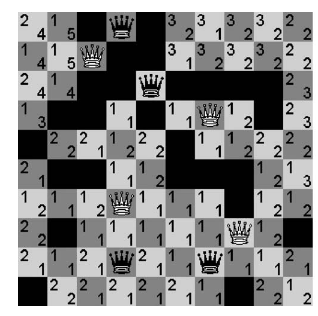
\includegraphics{exemple_territory}
	\caption{Exemple de table des distances (\href{https://core.ac.uk/download/pdf/81108035.pdf}{source})}
	\label{fig:exemple-territoire}
\end{figure}
\subsubsection{Optimisations supplémentaires}
On pourrait effectuer d'autres optimisations. Par exemple, on pourrait utiliser
une table de transposition, celle-ci s'occuperait de stocker l'évaluation connue pour un plateau.
Cela permettrait d'implémenter de l'Iterative Deepening de façon optimisée. L'Iterative Deepening consiste
à commencer à profondeur 1, et tant qu'il nous reste du temps, on passe à la profondeur suivante jusqu'à qu'on le temps soit écoulé.
Cependant, l'Iterative Deepening sans table de transposition revient à recalculer l'arbre à profondeur 1, ce qui est juste stupide. On pourrait
commencer l'exploration à partir du meilleur chemin trouvé. Au départ, nous avions comme intention
d'implémenter une table de transposition, mais par manque de temps nous avons dû abandonner.
